\chapter{Space and Coordinates}\label{ch:coordinates}

This chapter revises the basic concepts of common coordinate systems and their use in computer graphics. 
It also covers specific implementation details and conventions for representing vectors, transformations,
and other data structures in C/C++ and Vulkan/GLSL. 

This chapter assumes you are already familiar with the basic concepts of linear algebra, 
including vectors and matrices, trigonometry, and basic calculus.

\section{Common Coordinate Systems}\label{sec:common-coordinate-systems}

In simple terms, a coordinate system is a $1:1$ mapping from a geometric space $S$ to a set of real numbers $\mathbb{R}^n$.
It has a fixed origin or reference point, often defines a set of basis vectors also called axes, 
and defines a set of units or parameters to express the coordinates of a point in this space
(e.g. linear distances or angular  measurements).  
This section covers the most common coordinate systems and common operations on them\cite{arfken2012mathematical}.

\subsection{Cartesian Coordinates}\label{subsec:cartesian-coordinates}

Defined by a set of perpendicular axes, Cartesian coordinates are the most common system used to represent Euclidean geometry. 
It is widely used in everyday life, CAD, and physics.
It typically uses two or three dimensions, with the origin at the intersection of the axes.
The coordinates of a point are expressed as $(x,y)$ in 2D or $(x,y,z)$ in 3D, 
where $x$ (horizontal), $y$ (vertical), and $z$ (depth) are the linear distances from the origin along the respective axes. 

For any two points $P_1=(x_1,y_1,z_1)$ and $P_2=(x_2,y_2,z_2)$, 
the Euclidean distance between them is given by $d$:
\[
d(P_1,P_2)=\sqrt{(x_2-x_1)^2+(y_2-y_1)^2+(z_2-z_1)^2}
\]

Given two vectors $\mathbf{a}$ and $\mathbf{b}$, the dot product represents the cosine of the angle between them,
while the cross product represents a vector perpendicular to both.

\[
\mathbf{a}\cdot\mathbf{b} = |\mathbf{a}||\mathbf{b}|\cos\theta
\]
\[
\mathbf{a}\times\mathbf{b} = |\mathbf{a}||\mathbf{b}|\sin\theta \, \mathbf{n}
\]

The determinant of a $3\times 3$ matrix formed by three vectors $\mathbf{a}$, $\mathbf{b}$, and $\mathbf{c}$ 
gives the volume of the parallelepiped between them\cite{strang2016introduction,stewart2020calculus}:

\[
V = \det(\mathbf{a},\mathbf{b},\mathbf{c})
\]

To transform (translate, scale, and rotate) a point/vector in 3D space, 
a $4\times 4$ transformation matrix can be used. See Figure~\ref{eq:transformation-matrix}.
Note that the order of operations for matrix multiplication is not commutative.~\cite{strang2016introduction}

\begin{figure*}[!t]
\begin{align}
M_{\text{translate}} &= 
\begin{bmatrix} 
    1 & 0 & 0 & t_x \\ 0 & 1 & 0 & t_y \\ 0 & 0 & 1 & t_z \\ 0 & 0 & 0 & 1 
\end{bmatrix}
\\
M_{\text{scale}} &= 
\begin{bmatrix} 
    s_x & 0 & 0 & 0 \\ 0 & s_y & 0 & 0 \\ 0 & 0 & s_z & 0 \\ 0 & 0 & 0 & 1 
\end{bmatrix}
\\
M_{\text{rotate}} &= 
\begin{bmatrix} 
    \cos\alpha\cos\beta & \cos\alpha\sin\beta\sin\gamma - \sin\alpha\cos\gamma & \cos\alpha\sin\beta\cos\gamma + \sin\alpha\sin\gamma & 0 \\ 
    \sin\alpha\cos\beta & \sin\alpha\sin\beta\sin\gamma + \cos\alpha\cos\gamma & \sin\alpha\sin\beta\cos\gamma - \cos\alpha\sin\gamma & 0 \\ 
    -\sin\beta & \cos\beta\sin\gamma & \cos\beta\cos\gamma & 0 \\ 
    0 & 0 & 0 & 1 
\end{bmatrix}
\end{align}
\caption{Transformation matrices for Cartesian coordinates}
\label{eq:transformation-matrix}
\end{figure*}

\subsection{Polar Coordinates}\label{subsec:polar-coordinates}

A point in 2D polar coordinates is expressed as $(r,\theta)$,
where $r$ is the radial distance from the origin and $\theta$ is the angle measured counterclockwise from the positive $x$-axis.
The conversion between Cartesian and polar coordinates: 
$x = r\cos\theta$, $y = r\sin\theta$ and $r = \sqrt{x^2+y^2}$, $\theta = \arctan2(y,x)$.~\cite{arfken2012mathematical}

Polar coordinates are commonly used in physics and engineering for problems with circular symmetry, such as wave propagation.
They are also the basis for imaginary numbers and complex analysis, 
where a complex number $z$ can be represented as $z = re^{i\theta}$.

\subsection{Spherical Coordinates}\label{subsec:spherical-coordinates}

Similar to polar coordinates, a point in 3D spherical coordinates is expressed as $(r,\theta,\phi)$,
where $r$ is the radial distance from the origin, $\theta$ is the polar angle measured from the positive $z$-axis,
and $\phi$ is the azimuthal angle measured counterclockwise from the positive $x$-axis in the $xy$-plane.
See Figure~\ref{fig:spherical-coordinates}.
The conversion between Cartesian and spherical coordinates:
$x = r\sin\theta\cos\phi$,  $y = r\sin\theta\sin\phi$, $z = r\cos\theta$, and
$r = \sqrt{x^2+y^2+z^2}$, $\theta = \arccos(z/r)$, $\phi = \arctan2(y,x)$.~\cite{arfken2012mathematical}

\begin{figure}[htbp]
    \centering
    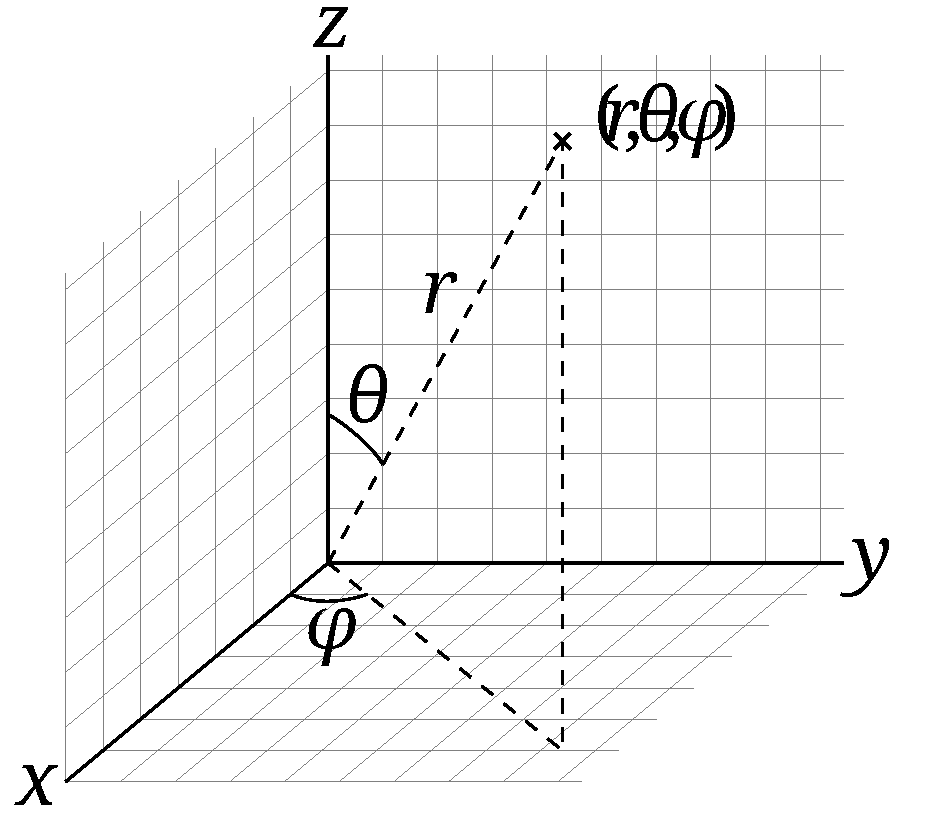
\includegraphics[width=0.75\columnwidth]{coordinates/3D_Spherical} 
    \caption{3D Spherical Coordinate System representation.}
    \label{fig:spherical-coordinates}
\end{figure}

\subsection{Schwarzschild Coordinates}\label{subsec:schwarzschild-coordinates}
\subsection{Eddington-Finkelstein Coordinates}\label{subsec:einstein-finkelstein-coordinates}
\subsection{Kruskal-Szekeres Coordinates}\label{subsec:kruskal-szekeres-coordinates}
\subsection{Painlevé-Gullstrand Coordinates}\label{subsec:painleve-gullstrand-coordinates}
\subsection{Boyer-Lindquist  Coordinates}\label{subsec:boyer-lindquist-coordinates}
\subsection{Kerr-Schild Coordinates}\label{subsec:kerr-schild-coordinates}
\subsection{Penrose Coordinates}\label{subsec:penrose-coordinates}


\section{The Jacobian}\label{sec:jacobian}

In multivariable calculus, 
the Jacobian is the basic mathematical framework for linearizing vector-valued functions 
and transforming coordinate systems. 
Depending on the context, the term Jacobian refers to either the matrix 
of first-order partial derivatives or to its corresponding determinant.~\cite{stewart2020calculus}

\subsection{The Jacobian Matrix}\label{subsec:jacobian-matrix}

The Jacobian matrix, 
denoted as $\mathbf{J}$ or $\frac{\partial(f_1, \dots, f_m)}{\partial(x_1, \dots, x_n)}$, 
is an $m \times n$ matrix of all possible first-order partial derivatives of $\mathbf{f}$. 
Each row corresponds to an output component function, and each column corresponds to an input variable:
\begin{equation}
    \mathbf{J} = \begin{pmatrix}
        \frac{\partial f_1}{\partial x_1} & \frac{\partial f_1}{\partial x_2} & \cdots & \frac{\partial f_1}{\partial x_n} \\
        \frac{\partial f_2}{\partial x_1} & \frac{\partial f_2}{\partial x_2} & \cdots & \frac{\partial f_2}{\partial x_n} \\
        \vdots & \vdots & \ddots & \vdots \\
        \frac{\partial f_m}{\partial x_1} & \frac{\partial f_m}{\partial x_2} & \cdots & \frac{\partial f_m}{\partial x_n}
    \end{pmatrix}
\end{equation}

Geometrically, 
the Jacobian matrix represents the best linear approximation of the function $\mathbf{f}$ 
in near a given point $\mathbf{p}$. 
It is the multivariable version of the single-variable derivative $f'(x)$.

\subsection{The Jacobian Determinant}
When a vector-valued function maps space to a space of the same dimension ($m = n$), 
the Jacobian matrix is a square. 
We can then compute its determinant:
\begin{equation}
    \det(\mathbf{J}) = \left| \frac{\partial(f_1, \dots, f_n)}{\partial(x_1, \dots, x_n)} \right|
\end{equation}

The Jacobian determinant represents the local \textit{space-scaling factor} of the transformation. 
It quantifies how much a small, differential volume or area expands, contracts, or flips orientation 
when processed through the function $\mathbf{f}$ at a specific location.

\subsection{Application: Change of Variables}
The primary analytical application of the Jacobian determinant is modifying boundaries and differentials 
during multivariable integration. (Change of variables theorem, used later).
When transitioning from a coordinate system $(x,y)$ to an alternative system $(u,v)$ via the transformations $x = x(u,v)$ 
and $y = y(u,v)$, the differential area element scales based on the absolute value of the Jacobian determinant:
\begin{equation}
    dx \, dy = \left| \det(\mathbf{J}) \right| du \, dv = \left| \frac{\partial x}{\partial u}\frac{\partial y}{\partial v} - \frac{\partial x}{\partial v}\frac{\partial y}{\partial u} \right| du \, dv
\end{equation}

Therefore, a double integral over a Cartesian region $R$ 
translates over a mapped region $G$ under the new coordinates as:
\begin{align}
    &\iint_R f(x, y) \, dx \, dy = \\
    &\iint_G f(x(u,v), y(u,v)) \left| \frac{\partial(x, y)}{\partial(u, v)} \right| du \, dv
\end{align}




\section{Calculus in Curvilinear Coordinates}\label{sec:calculus-in-curvilinear-coordinates}
\planned{$\nabla$, solid angle $\mathrm{d}\Omega=\sin\theta\,\mathrm{d}\theta\,\mathrm{d}\phi, \int_{\Omega}$}

\section{Rotations and Orientation}\label{sec:rotations-and-orientation}
\planned{$SO(3)$, axis--angle, Euler, quaternions, slerp, aligning a spin axis to $+z$}

\section{Homogeneous Coordinates and Projection}\label{sec:homogeneous-coordinates-and-projection}
\planned{affine maps, pinhole, NDC, camera-relative origin, perspective projection matrix, view matrix, model matrix}

\section{The Celestial Sphere\optmark}\label{sec:the-celestial-sphere}
\planned{equirectangular, cubemap, sampling distortion, HEALPix}


\section{Computer Hardware Limitations and Screen Space Conventions}\label{sec:computer-hardware-limitations-and-screen-space-conventions}

This section covers basic memory alignment and data layouts in C/C++ and GLSL, 
and compares the conventions used by different graphics APIs, programming languages, and hardware limitations.

\subsection{Memory Layouts and conventions}\label{subsec:memory-layouts}

The C and C++ compiler automatically aligns data structures in memory to optimize access speed.
\TODO{C compiler reference}

On the GPU side, the Vulkan specification defines three different memory layouts: 
\texttt{std140}, \texttt{std430}, and \texttt{scalar}. See Table~\ref{tab:memory-layouts} for a direct comparison.


\begin{table*}[htbp]
\centering
\caption{Direct Comparison of Vulkan Buffer Memory Layouts}
\label{tab:memory-layouts}
\begin{tabular}{p{4.4cm} p{3.6cm} p{3.6cm} p{3.6cm}}
\hline
\textbf{Feature / Member Type} & \textbf{\texttt{std140} (Extended)} & \textbf{\texttt{std430} (Base)} & \textbf{\texttt{scalar} (Scalar)} \\ \hline
\textbf{Primary Use Case} & Default for Uniform Buffer Objects (UBOs). & Default for Shader Storage Buffer Objects (SSBOs). & Highly dense, tightly packed structures. \\
\textbf{Vulkan Core Status} & Standard core behavior. & Core since Vulkan 1.2 (via standard layout extension). & Core since Vulkan 1.2 (via scalar block layout). \\
\textbf{Scalars (\texttt{float}, \texttt{int})} & Aligned to base size (4 bytes). & Aligned to base size (4 bytes). & Tightly packed to base size (4 bytes). \\
\textbf{Vectors (\texttt{vec2}, \texttt{vec4})} & \texttt{vec2} = 8B; \texttt{vec3}/\texttt{vec4} = 16B alignment. & \texttt{vec2} = 8B; \texttt{vec3}/\texttt{vec4} = 16B alignment. & Aligned to component base size (\texttt{vec3} takes 12B). \\
\textbf{Array Element Stride} & Rounded up to a multiple of a \texttt{vec4} (\textbf{16 bytes}). & Equal to the base alignment of the element type. & Equal to the exact size of the element type. \\
\textbf{Nested Struct Alignment} & Rounded up to a multiple of \textbf{16 bytes}. & Aligned to its largest member's alignment. & Aligned to the alignment of its single largest scalar element. \\
\textbf{Memory Efficiency} & \textbf{Low}: Prone to heavy padding and wasted bandwidth. & \textbf{Medium}: Efficient for arrays, but \texttt{vec3} still pads. & \textbf{Maximum}: Zero padding; matches native C/C++ packaging. \\ \hline
\end{tabular}
\end{table*}



\TODO{row vs column major order}

\TODO{host visible/coherent and PICe bus + VRAM vs UM}

\TODO{rebar}

\subsection{Screen Space}\label{subsec:screen-space}

Different graphics APIs use different conventions for screen space coordinates.
OpenGL and Vulkan use normalized device coordinates (NDC) in the range $[-1, 1]$ for both $x$ and $y$ axes
($[0, 0]$ at the center of the screen),
while Direct3D uses the range $[0, 1]$ for the $y$ axis
($[0, 0]$ at the bottom-left corner of the screen).
While Vulkan defines the origin of the screen space at the top-left corner ($+X$ right, $+Y$ down), 
OpenGL defines the origin at the bottom-left corner ($+X$ right, $+Y$ up).

